\documentclass[11pt]{article}

\usepackage[margin=1.0in]{geometry}
\usepackage{fullpage}
\usepackage{url}
\usepackage{paralist}
\usepackage[pdftex]{graphicx}
\usepackage{epstopdf}
\usepackage[small]{caption}
\usepackage{subfig}
\usepackage{multirow}
\usepackage{color}


%%% TO DO
%-- Methodology
%    -- more thoroughly explain nudging selection process (James)
%-- Evaluation
%    -- paragraph explaining scenario


% The xxx tag is intended to denote urgent text that needs addressing.
% The meh tag is intended to highlight text that needs some loving or which
% we're not sure should make primetime
\newcommand{\xxx}[1]{{\bf \color{red} #1}}
\newcommand{\meh}[1]{{\bf \color{blue} #1}}
\newcommand\T{\rule{0pt}{3ex}}
\newcommand\B{\rule[-1.2ex]{0pt}{0pt}}

\title{Reducing Uncertainty and Acquiring Knowledge Through Interaction}
\author{Rob Goeddel \and Lauren Hinkle \and James Kirk \and Aaron Mininger}
\date{}

\begin{document}
\maketitle


\begin{abstract}
When an agent is faced with uncertainty it has two major courses of action: it can explore on its own to gain more knowledge or it can consult an expert. We have created an image recognition system that utitilizes both sources of knowledge to improve its performance. Our system captures point-cloud data from an RGB-D camera and uses machine learning techniques to extract features and classify properties of objects including size, shape, and color. It is able to measure the amount of uncertainty for a given property and manipulate the object using a robotic arm in order to reduce that uncertainty. It also incorporates direct feedback from the user to further improve its classification performance and requests more information when it misclassifies an object. Users can easily teach the system new property labels on the fly. We demonstrate our system through a simple I-Spy game with toy blocks of various shapes and colors.
\end{abstract}


\section{Introduction}
%\xxx{Problem description and motivation. Why do you want to solve this
%    problem? What's the impact if you can solve this problem?}
Agents that operate in environments that are partially observable or very noisy are often faced with large amounts of uncertainty. One option for the agent is to explore the environment to resolve some of that uncertainty. While this approach can be done autonomously without direct human involvement, there still may be fundamental limits to what information the agent is able to collect. A second option is for the agent to consult an expert to acquire missing knowledge, a technique known as active learning. This can present a large and rich source of knowledge but can be costly to acquire. Hybrid approaches enable an agent to explore the world on its own and ask an expert for knowledge only when it needs to. This hybridization leverages the strengths of each option and can lead to better performance. Of course, intregrating them introduces new challenges such as how to tell when knowledge is unattainable through exploration or what consitutes an important question.

Our project involves one such attempt to utilize both sources of knowledge. Our system is tasked with identifying properties of various objects like color, shape, and size in order to play the children's game ``I-spy''. Unfortunately it is quite common for an object to be in a poor orientation and thus difficult for our system to classify. We use both recent history and information from our K-Nearst Neighbor (KNN) classifier to determine when we are uncertain about an object. Instead of asking the user for help, the system first tries to get more information about the object by nudging it using a robotic arm. The goal is to change the orientation of the object in order to improve its classification performance. It will learn which classes are inherintly uncertain (such as rectangles) and adjust accordingly. We also will ask for feedback from the user when an object is misidentified to gain more training data. Our system is flexible enough to allow users to teach new classes of properties during its operation.

This work is being incorporated in a larger project which includes teaching the
agent new concepts and actions. Such a project relies on having
symbolic information provided by our work through object segmentation and
classification. The low level features provided by our system can be analyzed and
combined in order to build new concepts such as object categories (like blocks
and balls) or object properties (all bananas are yellow). Such reasoning and
concept generalization is essential for agents that interact in novel situations.

The challenges involved in playing I Spy include object detection, feature
extraction, classification, robot arm manipulation, and active learning. We
discuss these further in Section 3.

\section{Related Work}
%\xxx{What are existing methods? What are the state-of-the-art methods for this
%    problem? How is your approach different from the related work?}

Our work spans a number of domains, with aspects similar to projects in image recognition, robotics, instruction, and active learning. There is a rich history of work in object recognition within computer vision, and some more recent efforts have focused on generalizing objects into classes like cars, bikes, or trucks ~\cite{huber2004parts}. Other work has focused on constructing more powerful classifiers built upon detecting aspects like color and shape from the image ~\cite{nilsback2006visual} ~\cite{gehler2009feature}. Recent popularization of sensors that combine both image and depth information like the Microsoft Kinect can provide richer sensory information to aid in vision tasks. Depth can make the determination of an object's underlying geometry much easier, leading to better identification ~\cite{marton2010hierarchical}. Other work has successfully incorporated such RGB-D cameras with object recognition in indoor domains featuring common household objects ~\cite{marton2010hierarchical, lai2011sparse}.

Our work combines both interacting with the world and using interaction to obtain more information. Most previous work focuses on one of the two sources. Some researchers have used robotic manipulation in order to discover information about an object like geometry, grasping points, and kinematics. Li and Kleeman created a system that nudged objects in order to improve its segmentation ~\cite{li2008autonomous}. Katz and Brock used a robotic arm to manipulate an object in order to obtain a kinematic model ~\cite{katz2008manipulating}. These systems do not integrate interaction from a user. Other systems do use human instruction to learn about the world, and several of those use robots and simple toy objects to learn about colors, shapes, and spatial relations. One system involved an environment very similar to ours, but only used the robotic arm for pointing, not manipulating ~\cite{skocaj2007system}. Another involved teaching a robot with foam blocks, but only used the robot to pick up an object once it recognized it ~\cite{zambuto2010visually}. The novelty of our project comes in utilizing both exploration through manipulating physical objects and human instruction to learn about the world. We believe that both sources have different strengths and that combining them can lead to improved learning abilities.

\section{Methodology}
%\xxx{How are you going to solve this problem? Why should the proposed method
%    work? Provide technical details of your approach if you are proposing a
%    novel method.}

\subsection{Point Cloud Acquisition}
Our work is intended to work with any colored 3D point cloud data. The
Microsoft Kinect is a simple and cost effective platform for acquiring
this data. We interface with the Kinect using the OpenKinect
library~\cite{OpenKinect}. The Kinect broadcasts LCM~\cite{huang2010} messages
containing orientation and frame information for other software to process.

Aligning color and depth data from the Kinect requires not only
calibrating the individual color and IR cameras, but also cross calibrating
the two. To do this, we explored several existing toolkits, eventually
using on RGBDemo~\cite{rgbdemo}. This kit automatically performs all of the
necessary calibrations, returning alignment parameters as well as terms for a
radial distortion model.

\subsection{Object Detection and Tracking}
In order to play I Spy, the agent must be able to point at objects matching the
provided description as well as nudge objects with low confidence in their
descriptions in order to see them from a new angle and gather new information
about them. In order for the agent to do this, it is necessary to have localized
positions for individual objects in the scene. Additionally, tracking objects
between frames allows confidence levels to change over time.

The RANSAC algorithm~\cite{fischler1981random} is used to discover the dominant
plane in each image, isolating most of the objects in the scene. Further
segmentation is performed to try to discover definitive object boundaries. This
segmentation considers both the change in color and change in depth of neighboring
pixels.
%Each pixel begins as its own segment, and the segments are iteratively
%combined with neighboring segments if the difference in color or the distance
%between them is less than a given threshold.
From these segmentations we extract a feature vector for each object.

In order to adjust the confidence thresholds to determine which shapes are more
certain (discussed below), it is necessary to track an object over time. This can
be challenging, as the physical object may change location over time or may be
occluded by the robot arm or another object. As each new frame appears, the
segmented objects in it are compared to prior segmented objects, beginning with
those of the most recent frame and continuing on to past frames if no matches are
found in the most recent. An object is matched to a prior object if the difference
in their mean color is small. The object is matched to the physically closest object
with a small enough difference in mean color that has not already been matched.

\subsection{Feature Extraction}

Once an object was segmented we extracted relevant features in order to classify
color, size, and shape. We considered objects that were of a single color, therefore
average red, green, blue, hue, saturation, and value levels across the pixels were
used as a six-dimensional feature vector. For size we calculated the diagonal of the 3D
axis-aligned bounding box and used that as one of our features. The second feature was
the average distance of the points from the centroid. Having the point-cloud data from
the Kinect allowed us to compute those features more accurately in three-dimensions
and saved us from having to do more complicated depth estimates.

Correctly classifying shapes required much more complicated features.
During this work we explored several options for extracting features from
objects before settling on the method described in this paper. We experimented
with ORB, a rotation invariant feature extractor similar to SIFT and SURF
~\cite{rublee2011orb}. Additionally we tested several feature detectors from
OpenCV, including their square detector~\cite{opencv_library}. We also explored
using RANSAC to discover simple shape types (such as planes, curves, and spheres),
in order to determine the number of faces and edges each object has. This work
was based off the RANSAC algorithms of Schnabel et
al~\cite{schnabel2007efficient}. Although these and other feature detectors are
frequently used in object recognition and learning tasks, we ultimately chose to
use our own Principal Component Analysis (PCA)-based method which resulted in
more accurate guesses from the agent than the other methods.

To extract edge features we apply PCA in order to find the axis the points were most spread out along.
For $N$ pixels we compute the mean pixel $\mu = \frac{1}{N}\displaystyle\sum_{i=1}^{N}x_i$. Then we find the covariance matrix $\Sigma = \frac{1}{N} BB^T$ where $B$ is an $N\times 2$ matrix with the $i$th column equal to $x_i - \mu$. The primay axis becomes the eigenvector with the largest eigenvalue. We then tranform the image into a canonical representation by finding a bounding box for the image aligned with the axes and rotating and scaling it to a unit box. To extract features we took evenly-spaced
points from the top and bottom edges of the box and calculated the vertical distance
from each point to the image. This process is illustrated by \subref{fig:pca}. We use seven
sample points along the top and bottom; experimental evaluation showed no significant
improvement with additional samples. In addition, we calculate the ratio of the width
and height before scaling to get an idea of how elongated the shape was. From each image we generated a total of four shape feature vectors after flipping the image vertically and horizontally. This allows us to more quicly learn a shape across different orientations.

\begin{figure}[h!]
\centering
    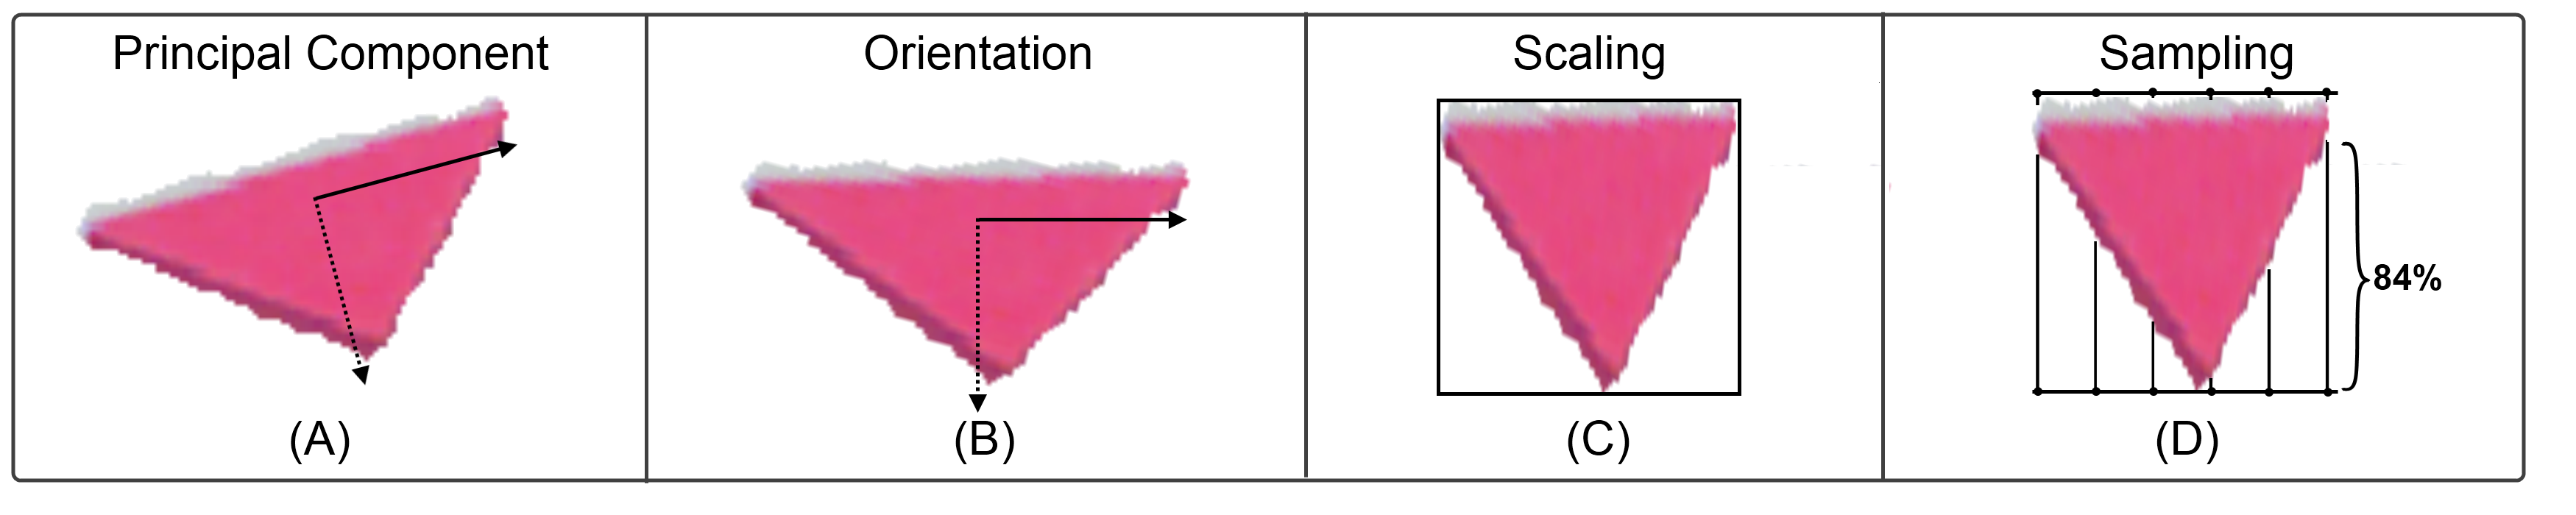
\includegraphics[width=1.0\textwidth]{figures/PCA_example.png}
    \caption{This figure illustrates using PCA to extract shape features. First the principal component is found (A), then the image is rotated and scaled accordingly (B, C). Finally, points are sampled along the top and bottom and for each the vertical distance to the image is recorded (D).}
    \label{fig:pca}
\end{figure}

\subsection{Classification}
Initially we used SVM classification to validate our method, but we have since
moved to a K-nearest neighbor approach.  With the KNN algorithm
it is easy to add another example to the training, without recreating the
entire training model as was done with SVM classification.  Additionally we no
longer rely on third party software, namely liblinear ~\cite{LIBLINEAR} to do
classification. KNN is also well suited for multiclass classification, removing
the need to do a one-vs-all (OVA) approach with multiple SVMs.  Adding a new
class to the KNN classifier is also easier and can be done dynamically. Using our
implementation of a K-nearest neighbor
classification we also reported a confidence metric for each label.

The confidence of a label is determined by calculating the percentage of K-nearest neighbors with that label.  The vision system experiences enough noise
to cause high variation in the classification, particularly when the
confidence is low.  To deal with this noise and stabilize the reported labels,
our system keeps track of the last 10 classifications, 15 for shape which is more noisy.  The K number for KNN chosen after some tuning similarly is 10 for size and color and 15 for shape.  The most popular label
is reported, with the confidence reported as the average confidence scaled by
the percentage of that label out of the ten.


\subsection{Confidence Thresholds and Object manipulation}
One of the difficulties with reasoning about real objects in the world is partially observability. Objects can have a dramatically different appearance at
different orientations. Naturally when given such an object, a human may move
his or her head around to gain more information and confidence as to what the object
is.  Similarly, when holding an unfamiliar object, a person may move it around
to further study it.

Our system has a fixed vision angle, but can
manipulate objects to gain information on those whose appearance has high
orientation dependency. For this purpose, a confidence threshold system was
developed to learn what objects may have high uncertainty, and therefore would
be good candidates for manipulation. When the system is queried for an object
that it cannot currently see, it should manipulate an uncertain object with the
highest probability of actually being the queried object.

All attributes are given the same default confidence threshold and adjusted
using user feedback. We attempt to estimate $P(label_{actual}(obj) \neq x | label_{observed}(obj) = x)$, which is the likelihood of a mislabel given the observed label $x$. For example, the rectangle label is commonly misapplied to objects presented head on. Thus our system learns a confidence threshold for rectangle is very high, meaning that $P(shape_{actual}(obj) \neq rectangle|shape_{observed}(obj) = rectangle)$ is very high. When the system it asked to identify an object by a given description it first tries to find an object that matches and points to it regardless of the confidence in the accuracy of the labels or the corresponding confidence thresholds. As a result, when the agent correctly identifies an object and the confidence is lower than the threshold for the given labels, those thresholds are lowered to reflect the correctness of the lower confidence. If there are no objects that match, it examines the labels in the same category to see if any object might be mislabeled. For each label it compares the confidence obtained from the KNN to that label's confidence threshold. If the confidence is lower, it will attempt to nudge that object in the hopes that the label is wrong. If multiple objects could be mislabeled it orders the search based on the difference between the confidences and the thresholds. When no objects are found matching the user description the thresholds are increased. In this case the agent prompts the user to identify the correct object. The thresholds for the reported labels should be increased, so that in the future the system will be more likely to attempt to manipulate objects with these labels and relvative confidences.

The thresholds are increased or decreased using the following formula:
$$\mathrm{Thresh_{t}} = \mathrm{Thresh_{t-1}}  \lambda^tdirection(t)$$
\[direction(t) = \left\{ \begin{array}{ll}
         1 & \mbox{if threshold should increase};\\
         -1 & \mbox{if threshold should decrease}.\end{array} \right. \]
where $t=$mathrm{number of times the threshold has changed.
\meh{My additions are okay, James should read over this and adjust to reflect
the actual code.I looked at it- still needs some review and equation explanation}

\subsection{Robot Arm Manipulation}
Our system is integrated with a robotic arm. The arm was loaned to us by Prof.
Edwin Olson and was developed for use in his undergraduate class. The arm
geometry is simple, allowing the use of closed form inverse kinematics solvers
for various positions.

Because the Kinect is not statically located with respect to the robotic arm,
we perform an initial manual calibration so we may align the Kinect coordinate
frame with that of the arm. All coordinates are transformed such that the arm
is centered at the origin facing down the x-axis at its default position. We
may command the arm to ``point'' or ``sweep'' at an object, prompting the arm
to execute a corresponding scripted action at the object location. Pointing is
self-explanatory. Sweeping causes the arm to execute a nudging action,
swinging the arm through the object at an angle to encourage rotation.

\subsection{Active Learning}
Active learning is the process with which an agent continues to adjust its
understanding of its environment by querying the user to gain information.
The I Spy agent utilizes the knowledge of the users playing the game with it
to continuously learn labels and improve its confidence about labels it has
already learned. The agent requests information from users when it makes an
incorrect object or when it cannot find the specified object. The labels the
user provides in response to the agent are added as training examples into the
KNN algorithm, as are all correct guesses that the user verifies.

The system is capable of begining with no knowledge and, through playing games
with people and requesting feedback about whether its guesses are correct or
incorrect, learn to distinguish shapes, colors, and sizes.

\section{Experimental Results}

\subsection{Data Collection and Training}
We acquired a large variety of children's foam blocks in many shapes, sizes,
and colors to act as our objects for classification. A small subset of the
blocks can be seen in Figure~\ref{fig:blocks}. The foam of the blocks is an
ideal material to work with as it
\begin{inparaenum}[(1)]
\item has a smooth, matte finish,
\item comes in a variety of distinct colors, and
\item is deformable enough to be grabbed by the arm but still retain its
shape.
\end{inparaenum}
Additionally we collected
more familiar objects to test our classifier on, demonstrating the ability of
the system to abstract general shapes to real world objects.

Our system, seen in figure \meh{screenshot}, segments objects found in the
predefined play area and labels them with the most confident shape, size, and
color.  Additionally a user can train new shapes, colors, and sizes by simply
clicking on that image and supplying the relevant label.  This is sufficient
for creating a large number of training samples, preferably at different
positions and orientations.  This method is not efficient for generating a
large number of training samples of many different objects, so we collected a
training dataset of footage of the foam blocks at numerous positions and angles
throughout the play area which were then segmented and labeled with relevant
descriptors.  Our training data consisted of 1812 shape examples, 1889 color exmaples, and \meh{number} size examples;


\begin{figure}[h!]
\centering
\subfloat[Foam Blocks] {
    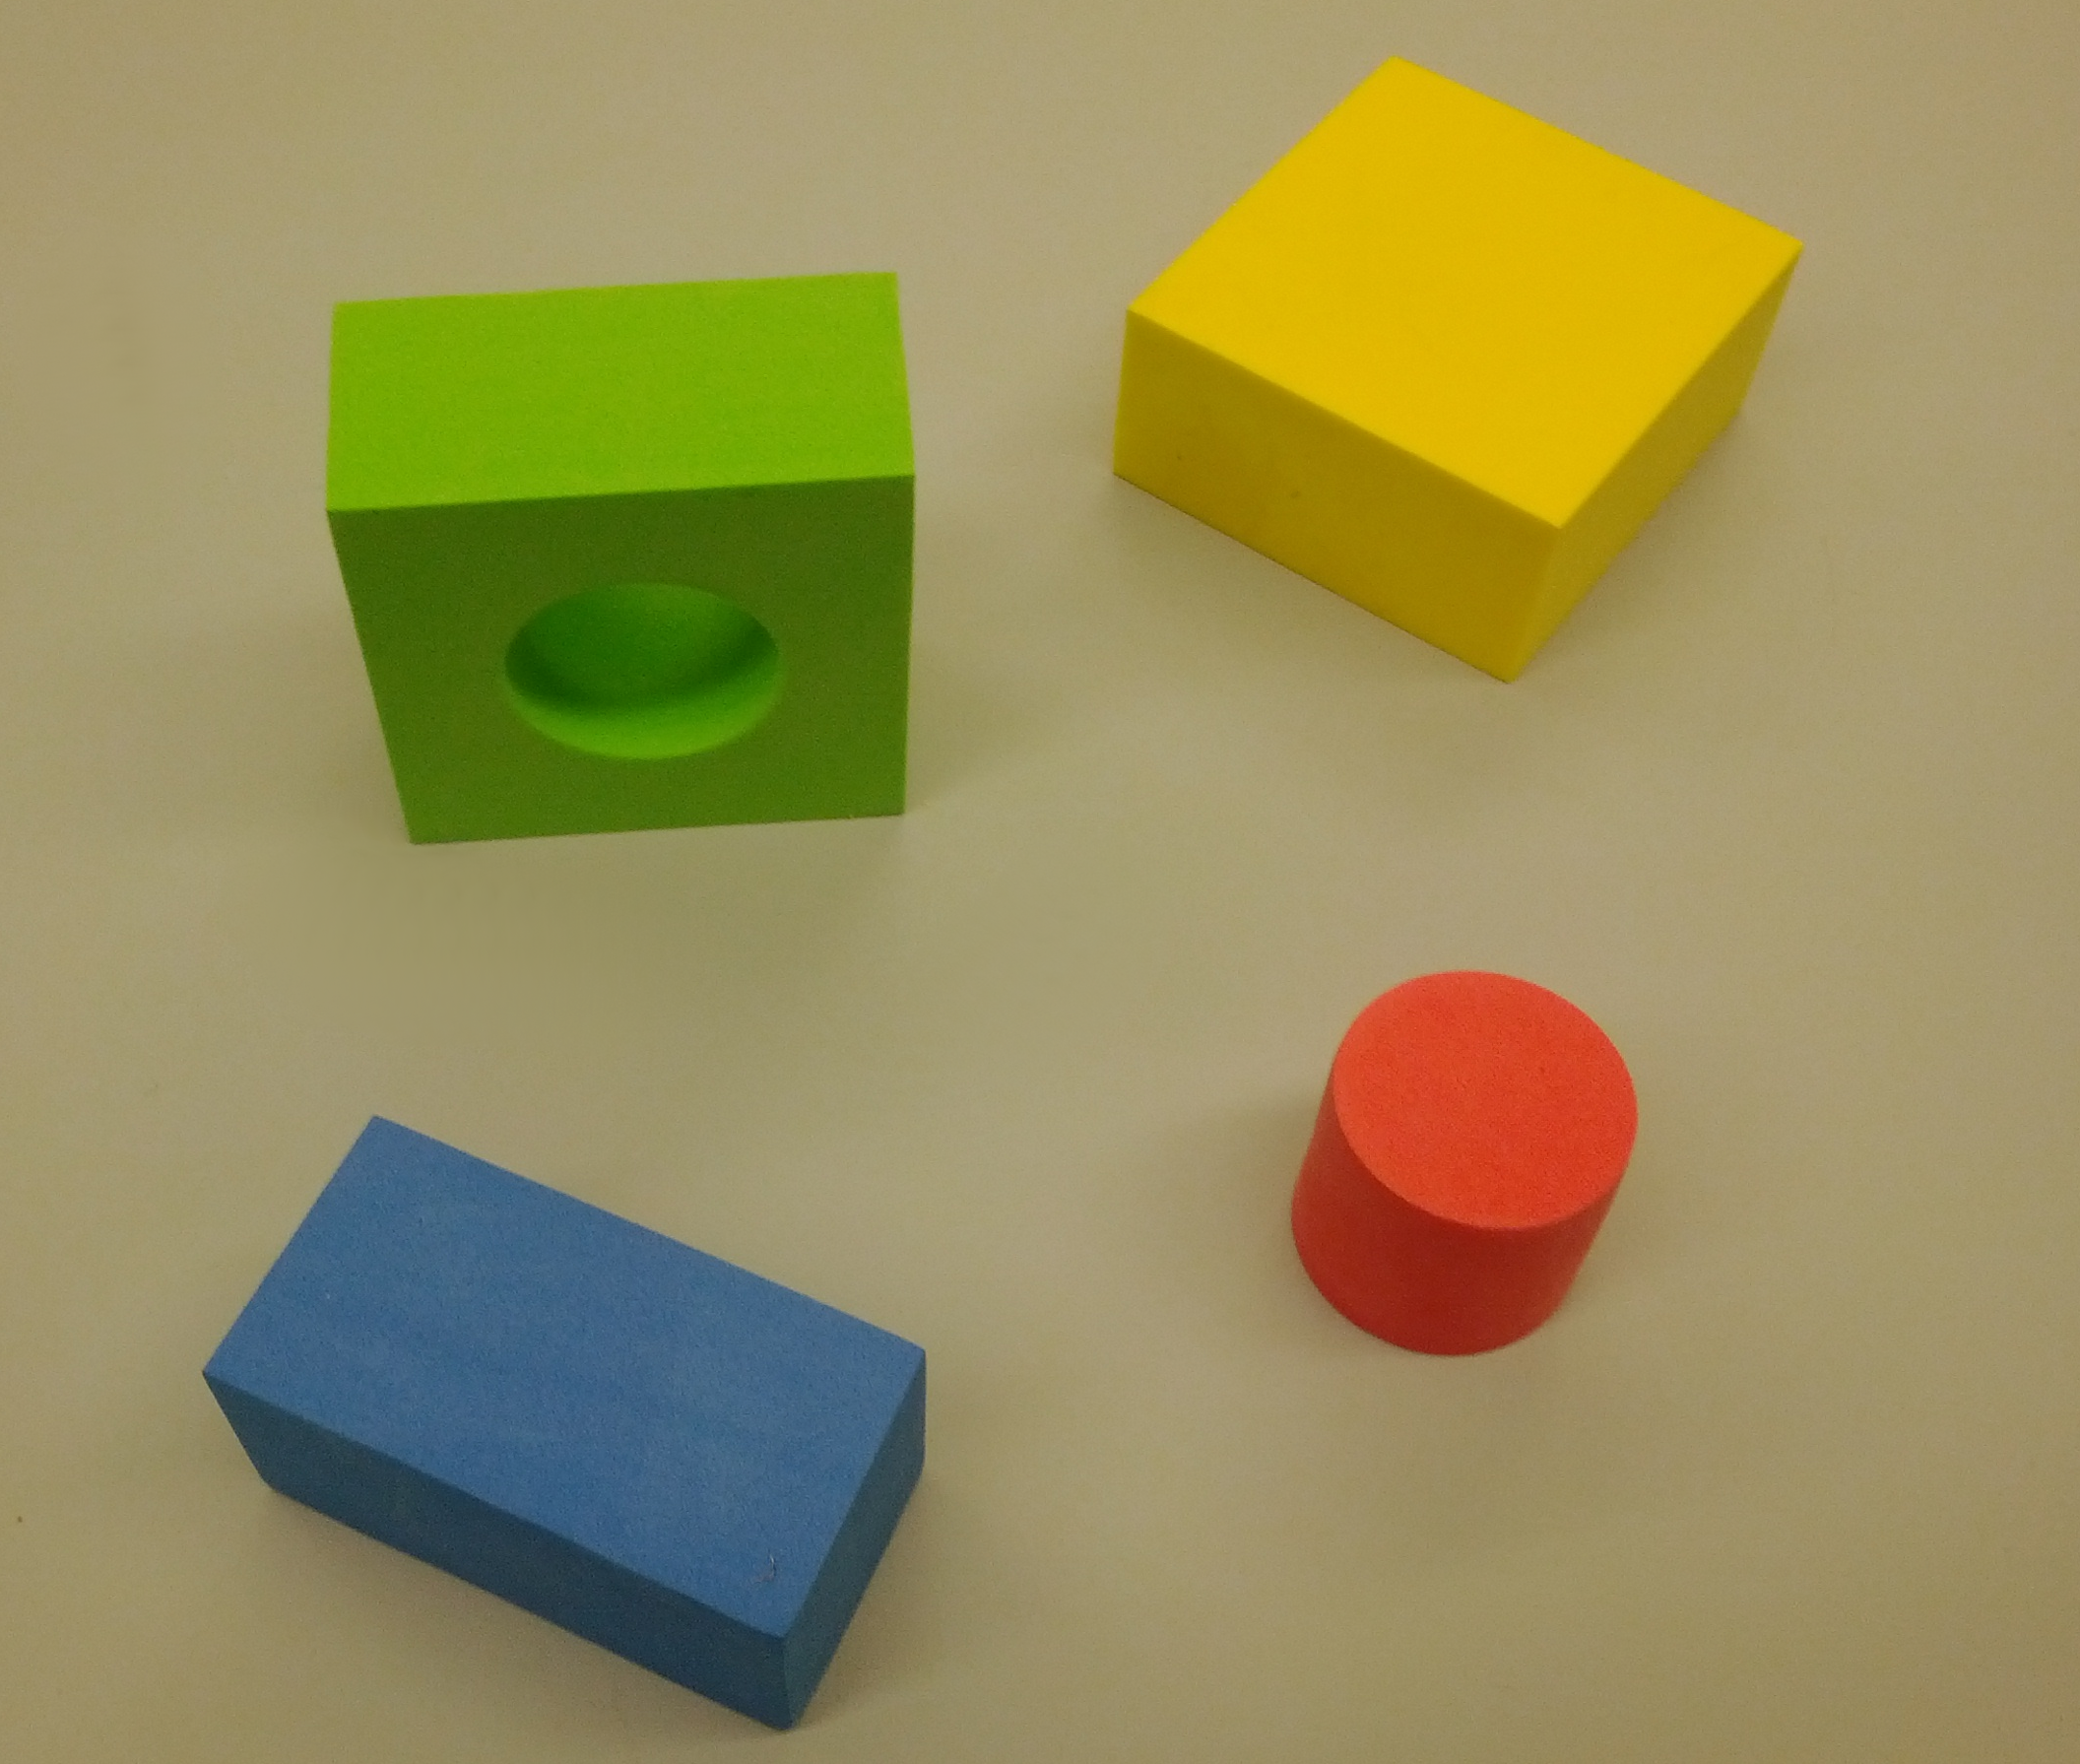
\includegraphics[height=1.6in]{figures/blocks.png}
    \label{fig:blocks}
}
\subfloat[Segmented Images] {
    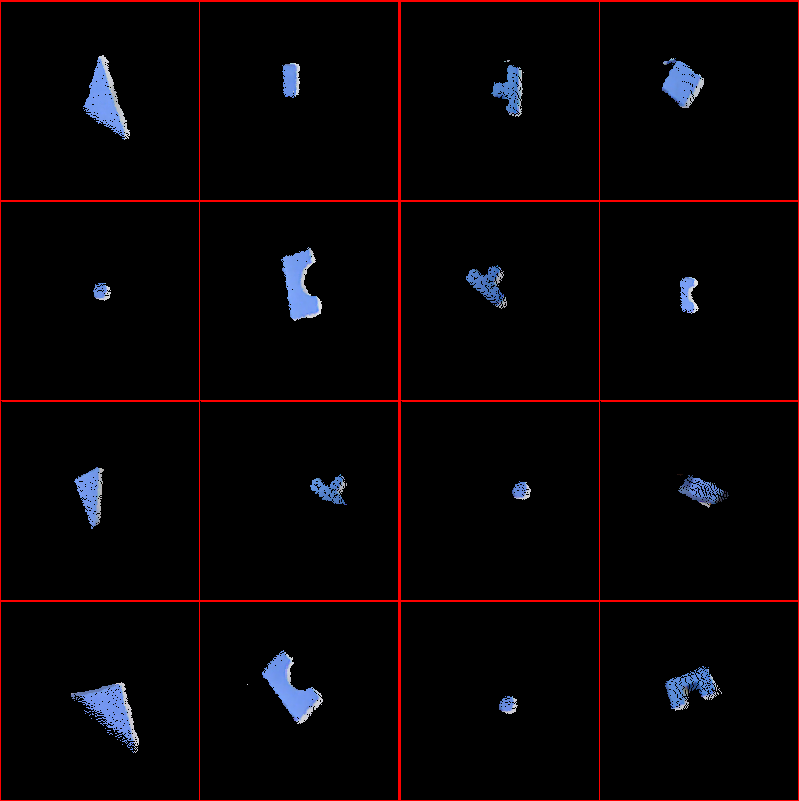
\includegraphics[height=1.6in]{figures/blue_objs.png}
    \label{fig:images}
}
\subfloat[Real-world test data] {
    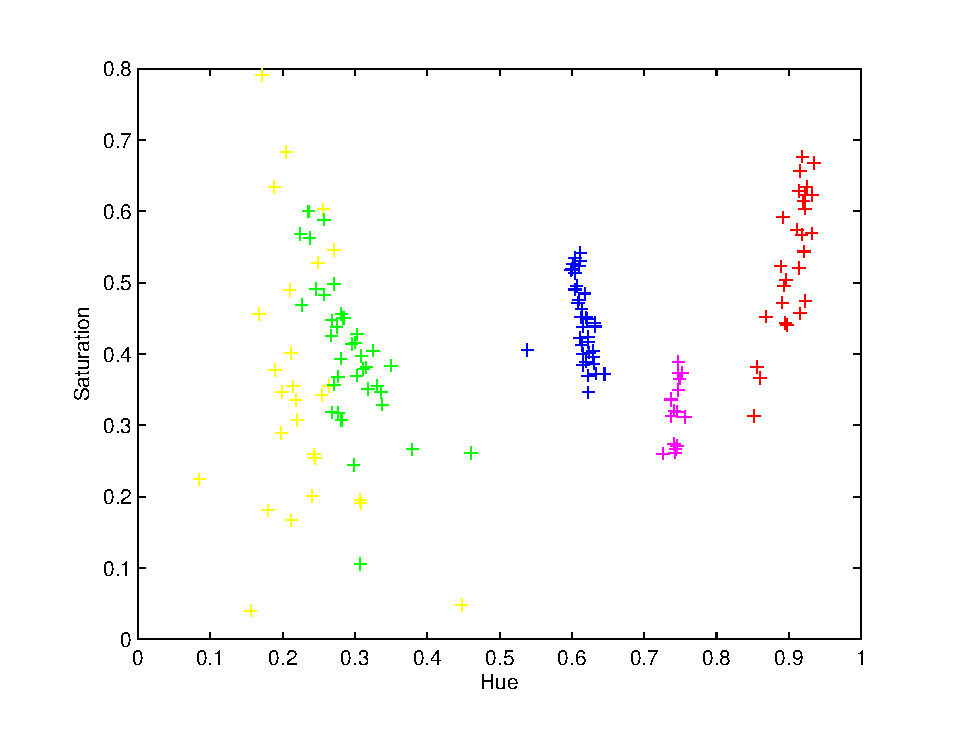
\includegraphics[height=1.6in]{figures/colorplot_noorange.eps}
    \label{fig:colordata}
}
\caption{Real world data is extracted from toy foam blocks. The blocks
    themselves can be seen in \subref{fig:blocks}. Using a segmentation
    algorithm, we extract the blocks from the Kinect data \subref{fig:images}
    and generate feature vectors for each object.
    Finally, we hand label the data for features such as color and shape for
    classification training. In \subref{fig:colordata}, we see the actual
    distribution of our training samples in the hue and saturation
    dimensions.}
\label{fig:objects}
\end{figure}


Real world data is extracted from toy foam blocks. The blocks
    themselves can be seen in \subref{fig:blocks}. Using a segmentation
    algorithm, we extract the blocks from the Kinect data \subref{fig:images}
    and generate feature vectors for each object.
    Finally, we hand label the data for features such as color and shape for
    classification training. In \subref{fig:colordata}, we see the actual
    distribution of our training samples in the hue and saturation
    dimensions.


Testing our system requires direct interaction and presentation of new objects
or objects at new angles.  Additional testing can be done by training the
system with new shapes and colors and observing how quickly and effectively it
can learn and apply the new information.  Qualitatively it is easy to see
whether the system is performing well.  However to do a less subjective,
quantitative evaluation of our methodology, we used the
leave-one-out-cross-validation(LOOCV) method on our collected training data. This
testing method mirrors the scenario where a novel object is presented to this
system.

The results in Table~\ref{tbl:testresults} \xxx{todo} show LOOCV percentages
for the shape, color and size.  Unsurprisingly it has more difficulty with shape,
which varies greatly by angle and position, and size, which is a more
subjective attribute. It has particular problems with shapes that are presented
head on, which tend to resemble rectangles.  This is the primary motivation for
developing a confidence threshold learning mechanism, which allows the system
to determine which labels are inherently uninformative.


% orange 87.10
\begin{table}
\centering
\begin{tabular}{ | l | l | l | l | l | l |}
    \hline
    shape &  size & color \T \B \\ \hline
    90.3\%  & 85.0\% & 99.7 \% \B \T \\ \hline
\end{tabular}
\caption{This shows the result of OVA classification for five color types
    across 160 objects. Each test involved training on 80\% of the points,
           with 20\% left out for testing.}
\label{tbl:testresults}
\end{table}

\section{Future Work}
This work is part of a larger project, Broad Operational Language Translation
(BOLT), is a joint undertaking by John Laird, Edwin Olson, and SoarTech and is
funded by DARPA. The goal of BOLT is to create a machine that can handle
situated interactive instruction with learned objects and actions. Our work has
focus on the needed feature learning and object classification that the BOLT
system will use.

The short term goals of this continued work involve further manipulation of the
objects such as picking them up in order to view them from different angles and
place them in different positions in the play area. Additionally we will be
interfacing our work with the SOAR archtecture. We had initially planned to
integrate SOAR in this project, but found that it decided it did not contribute
to the immediate goals of the project.

\section{Conclusion}
%\xxx{Summary of your progress and your final expected goal (what do you expect
%    to achieve or demonstrate for the final project?)}
In order to play I Spy, an agent must be able to correctly identify labels
associated with objects in its envronment. This requires identifiying objects
and their salient features, using prior knowledge to map features to labels, and
learning from mistakes in order to perform better in the future. We create an
agent that is capable of doing all of this, using a robotic arm to interact with
objects, a confidence threshold based system to dictate interaction choices, and
an interface that that allows it to actively learn from the user it is playing
with. The resulting system is the beginning of a more complex agent that can
use interaction with both users and its environment to gain a better understanding
of objects, labels, and semantics.


\bibliographystyle{abbrv}
\bibliography{literature}

\end{document}

% LocalWords:  multiclass
